\documentclass{beamer}

\usepackage{graphicx}
\usepackage{amsmath, amssymb, amsfonts}
\usepackage{listings} % For code inclusion
\usepackage{xcolor} % For color in code

\title{Solution to System of Equations}
\author{EE24BTECH11011 - B. Pranay Kumar}
\date{}

% Setup for code listings
\lstset{
    basicstyle=\ttfamily\small,
    keywordstyle=\color{blue},
    commentstyle=\color{green!50!black},
    stringstyle=\color{purple},
    showstringspaces=false,
    breaklines=true
}

\begin{document}

\frame{\titlepage}

\begin{frame}
    \frametitle{Problem Statement}
    Find the solution of the system of equations:
    \begin{align}
        \frac{3}{x} + \frac{8}{y} &= -1, \\
        \frac{1}{x} - \frac{2}{y} &= 2, \quad x, y \neq 0.
    \end{align}
\end{frame}

\begin{frame}
    \frametitle{Variable Substitution}
    To simplify, let:
    \begin{align*}
        a &= \frac{1}{x}, \\
        b &= \frac{1}{y}.
    \end{align*}
    The equations then become:
    \begin{align}
        3a + 8b &= -1, \\
        a - 2b &= 2.
    \end{align}
\end{frame}

\begin{frame}
    \frametitle{Matrix Representation of the Problem}
    We can represent the system in matrix form as:
    \[
    \begin{pmatrix} 3 & 8 \\ 1 & -2 \end{pmatrix} \begin{pmatrix} a \\ b \end{pmatrix} = \begin{pmatrix} -1 \\ 2 \end{pmatrix}
    \]
\end{frame}

\begin{frame}
    \frametitle{Solving Using Row Operations}
    Performing row operations to solve for \(a\) and \(b\):
    \[
    \begin{pmatrix} 3 & 8 & -1 \\ 1 & -2 & 2 \end{pmatrix}
    \xrightarrow{R_2 \rightarrow 3R_2 - R_1}
    \begin{pmatrix} 3 & 8 & -1 \\ 0 & -14 & 7 \end{pmatrix}
    \]
    Then,
    \[
    \begin{pmatrix} 3 & 8 & -1 \\ 0 & -14 & 7 \end{pmatrix}
    \xrightarrow{R_2 \rightarrow \frac{R_2}{-7}}
    \begin{pmatrix} 3 & 8 & -1 \\ 0 & 2 & -1 \end{pmatrix}
    \]
    \[
    \xrightarrow{R_1 \rightarrow R_1 - 4R_2}
    \begin{pmatrix} 3 & 0 & 3 \\ 0 & 2 & -1 \end{pmatrix}
    \]
\end{frame}

\begin{frame}
    \frametitle{Final Solution}
    The matrix simplifies to:
    \[
    \begin{pmatrix} 1 & 0 & 1 \\ 0 & 1 & -\frac{1}{2} \end{pmatrix}
    \]
    This gives:
    \begin{align*}
        a &= 1, \\
        b &= -\frac{1}{2}.
    \end{align*}
    Since \( a = \frac{1}{x} \) and \( b = \frac{1}{y} \), we find:
    \[
    x = 1, \quad y = -2.
    \]
\end{frame}

\begin{frame}[fragile]
    \frametitle{C Code for Calculating Points}
    The following C code calculates points for both equations to plot:
    \begin{lstlisting}[language=C]
    #include <stdio.h>
    #include <stdlib.h>
    #include <math.h>
    #include "libs/matfun.h"
    #include "libs/geofun.h"

    double calculate_y1(double x) {
        if (x == 0) return 0; 
        return 8 / (-1 - (3 / x));
    }

    double calculate_y2(double x) {
        if (x == 0) return 0;
        return 2 / (1/x - 2);
    }

    void plotPointsToFile(const char *filename, double **points, int num_points) {
        FILE *file = fopen(filename, "w");
        for (int i = 0; i < num_points; ++i) {
            fprintf(file, "%lf %lf\n", points[i][0], points[i][1]);
        }
        fclose(file);
    }
    \end{lstlisting}
\end{frame}

\begin{frame}[fragile]
    \frametitle{C Code for Generating Data Files}
    Main function to generate data files for plotting:
    \begin{lstlisting}[language=C]
    int main() {
        double x_start = -10.0, x_end = 10.0, step = 0.1;
        int num_points = (int)((x_end - x_start) / step) + 1;
        double **points1 = createMat(num_points, 2);
        double **points2 = createMat(num_points, 2);
        
        if (points1 == NULL || points2 == NULL) {
            printf("Error: Memory allocation failed.\n");
            return 1;
        }

        int index = 0;
        for (double x = x_start; x <= x_end; x += step) {
            if (x == 0) continue;

            points1[index][0] = x;
            points1[index][1] = calculate_y1(x);

            points2[index][0] = x;
            points2[index][1] = calculate_y2(x);

            index++;
        }

        plotPointsToFile("plot1.txt", points1, num_points);
        plotPointsToFile("plot2.txt", points2, num_points);

        freeMat(points1, num_points);
        freeMat(points2, num_points);
        return 0;
    }
    \end{lstlisting}
\end{frame}

\begin{frame}[fragile]
    \frametitle{Python Code for Plotting}
    This Python code reads the data files and plots the functions and intersection:
    \begin{lstlisting}[language=Python]
    import numpy as np
    from scipy.optimize import fsolve
    import matplotlib.pyplot as plt

    def equations(vars):
        x, y = vars
        return [(3 / x) + (8 / y) + 1, (1 / x) - (2 / y) - 2]

    guesses = [(1, 1), (-1, -1)]
    intersection_points = [fsolve(equations, guess) for guess in guesses]

    def read_points(filename):
        x_points, y_points = [], []
        with open(filename, 'r') as file:
            for line in file:
                x, y = map(float, line.split())
                x_points.append(x)
                y_points.append(y)
        return x_points, y_points

    x1, y1 = read_points('plot1.txt')
    x2, y2 = read_points('plot2.txt')

    plt.plot(x1, y1, label=r"$\frac{3}{x} + \frac{8}{y} = -1$")
    plt.plot(x2, y2, label=r"$\frac{1}{x} - \frac{2}{y} = 2$")
    for (x_int, y_int) in intersection_points:
        plt.plot(x_int, y_int, 'o', color='black')
    plt.axis([-10, 10, -10, 10])
    plt.legend()
    plt.show()
    \end{lstlisting}
\end{frame}

\begin{frame}
    \frametitle{Graphical Solution}
    \begin{figure}
        \centering
        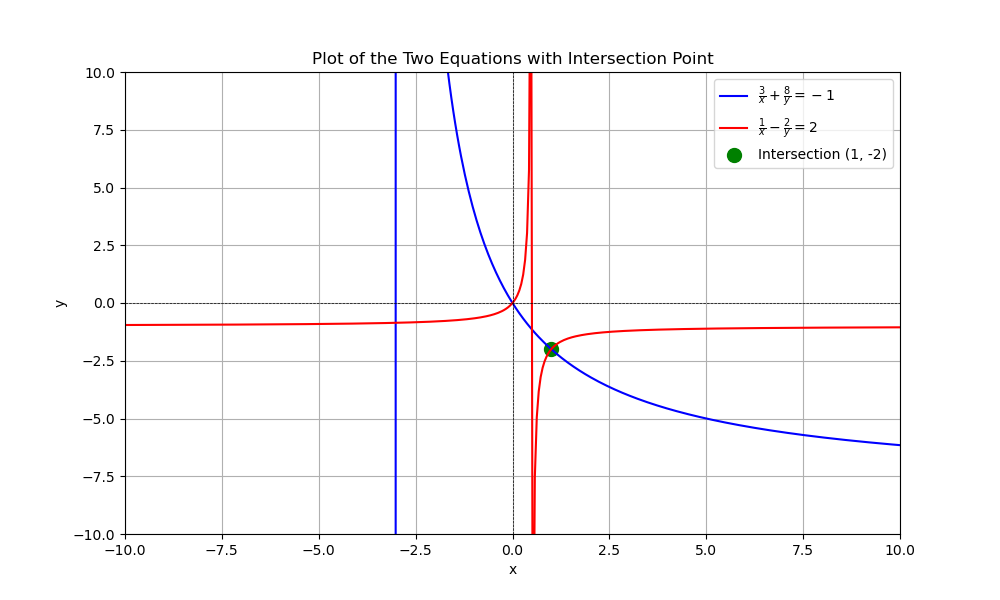
\includegraphics[width=0.7\linewidth]{figs/Q3.png}
        \caption{Graphical representation of the system of equations}
    \end{figure}
\end{frame}

\end{document}

